\chapter{Evaluation on a corporate dataset}\label{chap:cisco-dataset}

The tree methods were finally evaluated on a corporate dataset in the domain of computer security.

\section{The used dataset}

The models were evaluated on a proprietary dataset provided by Cisco Cognitive Intelligence, consisting of records of network connections from clients (e.g. user computers or mobile devices) to some on-line services. The dataset represents HTTP traffic of more than 100 companies. Two datasets were collected, each spanning 1 day of traffic. The training data was traffic from 2019-11-18, while the data used for testing was collected the following day, 2019-11-19. For each connection, a proprietary classification system based on \cite{jusko_graph-based_2017} provided labels, classifying the connections either as legitimate or malicious (connected to malware activity). The data was sampled to include 90\% of negative bags and 10\% of positive bags.

The dataset contained the following information for each connection:
\begin{enumerate}
  \item The duration of the connection, that is the difference between the time of the first and the last recorded datagram
  \item The client port number
  \item The IANA assigned internet protocol number
  \item The server port number
  \item The number of bytes sent from the client to the server
  \item The number of bytes sent from the server to the client
  \item The number of packets sent from the client to the server
  \item The number of packets sent from the server to the client
  \item The number of individual TCP connections
  \item The number of SYN packets sent from the client to the server
  \item The number of SYN-ACK packets sent from the server to the client
  \item The number of RST packets sent from the client to the server
  \item The number of RST packets sent from the server to the client
  \item The number of FIN packets sent from the client to the server
  \item The number of FIN packets sent from the server to the client
\end{enumerate}

In addition to that, each connection contains the URL the client is connecting to. A hierarchical representation of the URL using MIL was added to the features -- the MIL framework is powerful enough to enable a mix of traditional and MIL-based features. The URL model is based on the previous works \cite{dedic_hierarchicke_2017} and \cite{pevny_nested_2020}. The hierarchical model is visualized in figure \ref{fig:URL-model}.


\begin{figure}[h]
  \centering
  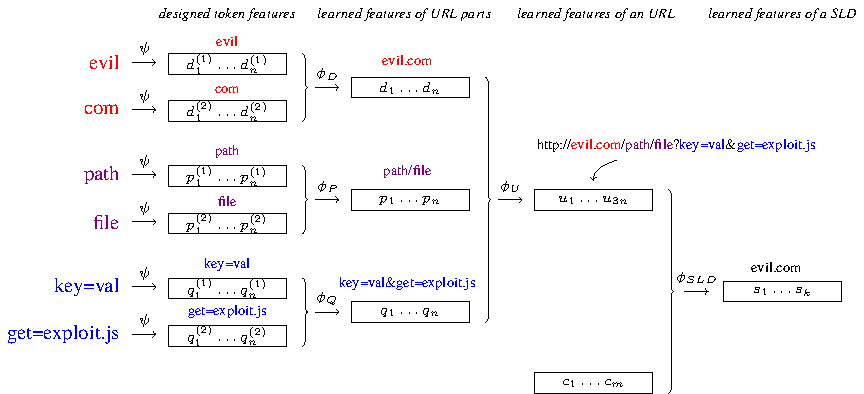
\includegraphics[width=\textwidth]{images/URL-model/URL-model.pdf}
  \caption{Hierarchical model of a URL. The vector \( c_1, \dots, c_m \) represents the connection features.}\label{fig:URL-model}
\end{figure}

\section{Used models}

The models for evaluation were implemented in the Julia programming language (see \cite{bezanson_julia:_2017}) using the Flux.jl framework for machine learning (see \cite{innes_flux:_2018}) and the Mill.jl framework for multi-instance learning (see \cite{pevny_milljl_2019}).

The embedding \( \phi \) was realised by a MIL neural network. Using the notation from figure \ref{fig:URL-model}, \( \phi_D \), \( \phi_P \) and \( \phi_Q \) consisted of a layer of 20 neurons, followed by concatenating element-wise mean and element-wise maximum of all instances in a bag. After joining the URL parts by concatenating their representations,\( \phi_U \) consisted of a layer of 120 neurons, followed by concatenation with the 15 connection features. Finally, \( \phi_\mathrm{SLD} \) consist of a layer of 135 neurons, followed by aggregation by concatenating element-wise mean and element-wise maximum of all instances in a bag, followed by a layer with 270 neurons. All the neurons used the ReLU activation function (see \cite{hahnloser_digital_2000}). Layer weights were initialized using Glorot initialization (see \cite{glorot_understanding_2010}), bias vectors were initialized to zeros. ADAM (see \cite{kingma_adam:_2014}) was used as the optimization method. The models were trained using 20 mini-batches of 50 bags each.

A mean model and a classification model have been constructed similarily to the ones in section \ref{sec:baseline-models}
The classification model is identical, with a final output layer of 2 neurons added. ADAM was used as the optimization method optimizing the cross-entropy loss. The accuracy of the model has been evaluated by selecting the optimal threshold on its output.

\section{Multi-class classification}
Apart from the task of learning a clustering based on a two-class labeling of bags as either legitimate or malicious, a multi-class classification system was also trained and evaluated. In this case, the data points were labeled as belonging to one of the following 20 classes of malware:

\begin{enumerate}
  \item Legitimate traffic
  \item Ad injector
  \item Anonymization software
  \item Advanced Persistent Threat (APT)
  \item Banking trojan
  \item Click fraud
  \item Cryptocurrency miner
  \item Data exfiltration
  \item Exploit kit
  \item Information stealer
  \item Malicious advertising
  \item Malicious content distribution
  \item Malware distribution
  \item Money scam
  \item Potentially unwanted application (PUA)
  \item Ransomware
  \item Scareware
  \item Spam botnet
  \item Spam tracking
  \item Trojan
\end{enumerate}

The data was sampled to include 81\% of legitimate bags and 1\% of every other class.

\section{Method comparison}

Figure \ref{fig:cisco-ratio} shows the value of \( \mathrm{ratio} \left( \cdot \right) \) for all the methods over the learning period. Figures \ref{fig:cisco-accuracy} and \ref{fig:cisco-kNN} show the accuracy of a kNN model built on the embedding.

Figure \ref{fig:cisco-multiclass-ratio} shows the value of \( \mathrm{ratio} \left( \cdot \right) \) for all the methods over the learning period for the 20-class classification problem. Figures \ref{fig:cisco-multiclass-accuracy} and \ref{fig:cisco-multiclass-kNN} show the accuracy of a kNN model built on the embedding. \todo{Add the figures}

\begin{figure}[h]
  \centering
  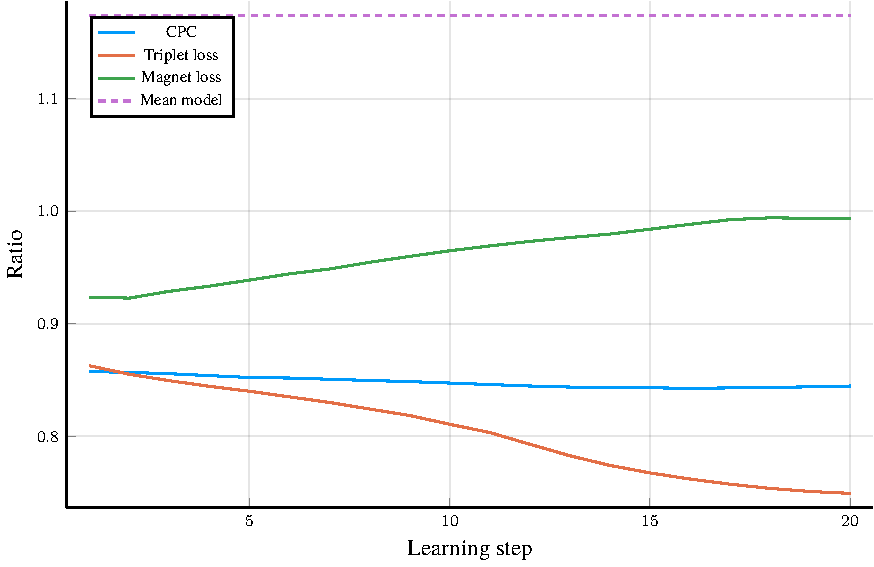
\includegraphics[width=\textwidth]{images/cisco/ratio/cisco-ratio.pdf}
  \caption{The value of \( \mathrm{ratio} \left( \cdot \right) \) for magnet loss over the learning period. Note the logarithmic scale on the \( y \) axis.}\label{fig:cisco-ratio}
\end{figure}

\begin{figure}[h]
  \centering
  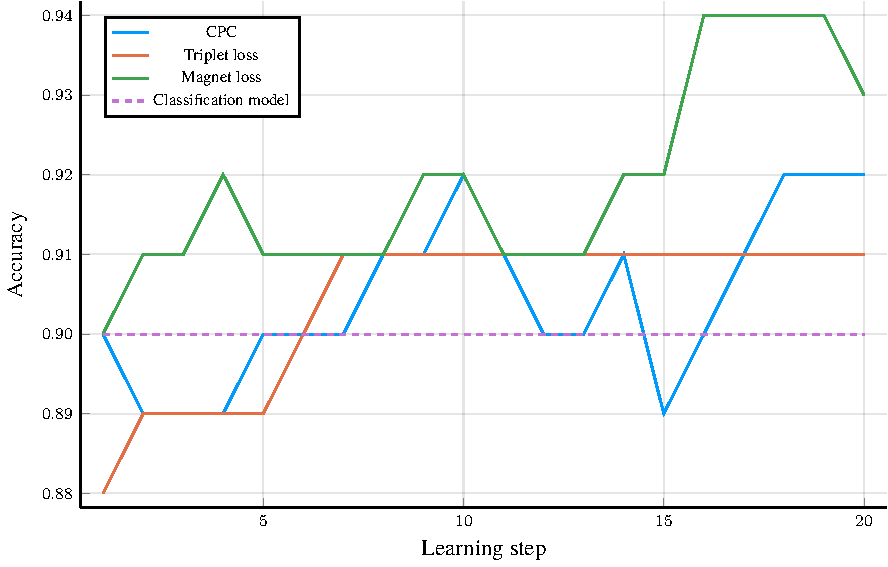
\includegraphics[width=\textwidth]{images/cisco/accuracy/cisco-accuracy.pdf}
  \caption{The accuracy of a kNN classifier built on the embedding for magnet loss over the learning period.}\label{fig:cisco-accuracy}
\end{figure}

\begin{figure}[h]
  \centering
  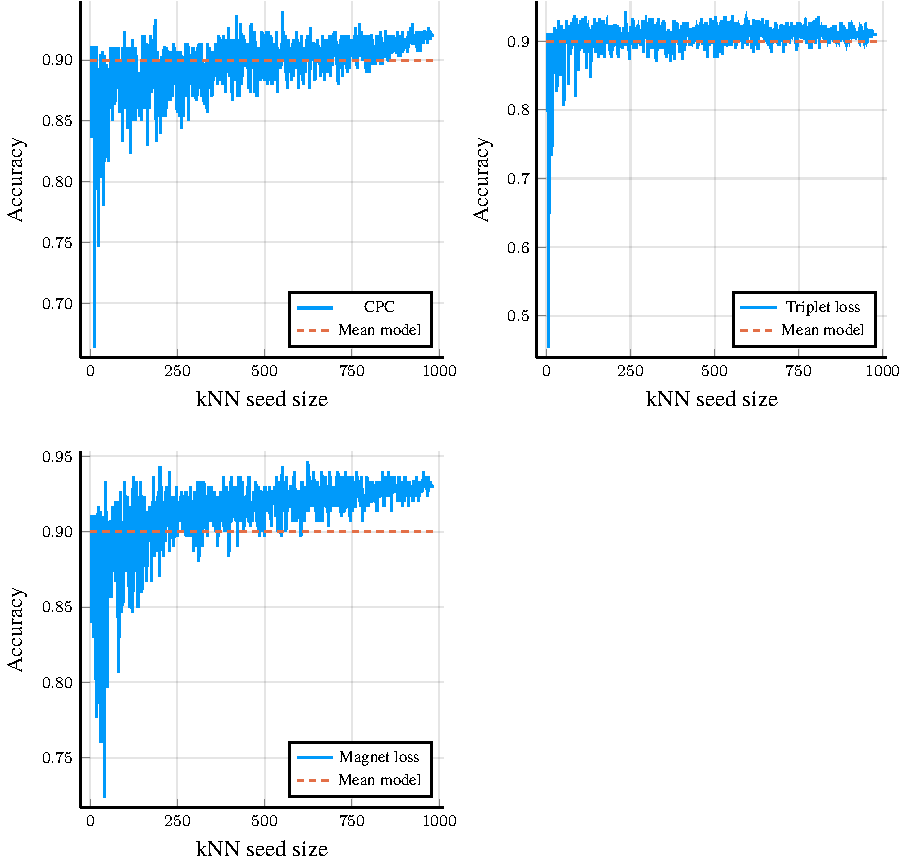
\includegraphics[width=\textwidth]{images/cisco/kNN/cisco-kNN.pdf}
  \caption{The accuracy of a kNN classifier built on the final embedding for magnet loss as a function of the number of samples used to seed it. Average of three runs.}\label{fig:cisco-kNN}
\end{figure}

As can be seen from the figures, for this problem, magnet loss performed the best. The model based on contrastive predictive coding is very unstable and while the model based on triplet loss increases its accuracy, the value of \( \mathrm{ratio} \left( \cdot \right) \) actually goes down over the learning period. Figure \ref{fig:cisco-kNN} shows that all of the methods reach their peak performance for a small number of seed data, but all three methods are very sensitive to the choice of the seed data. \todo{Multiclass}
